\documentclass{beamer}
%%% ========== Package setup ==========
\usepackage{xeCJK}      % Chinese words package
\usepackage{fontspec}   % Word fonts package
\usepackage{listings}   % Wrap Figure or table package
\usepackage{wrapfig}    % Multicolumn package
\usepackage{multicol}   % Multicolumn package
\usepackage{pdflscape}  % Landscpae package
\usepackage{tikz}       % TikZ picture package(Docs: https://ftp.ntou.edu.tw/ctan/graphics/pgf/base/doc/pgfmanual.pdf)
\usepackage[outline]{contour} % glow around text
\usepackage{amsmath}
\usepackage{mathtools}

%%% ========== Slide setting ==========
%% Slide theme setup
\usetheme{CambridgeUS}
\usecolortheme{wolverine}

%% Setup chinese words encoder
\XeTeXlinebreaklocale "zh"
\XeTeXlinebreakskip = 0pt plus 1pt

%% More word fonts
\setmainfont{Times New Roman}
\renewcommand{\familydefault}{\rmdefault}
\setCJKmainfont{標楷體}

% Setting for figure and table numbering
\setbeamertemplate{caption}[numbered]

% TikZ setting
\usetikzlibrary{positioning}
\usetikzlibrary{calc}
\usetikzlibrary{arrows.meta}

%%% ========== Title setup ==========
\date{September, 2022}
\title{Meeting}
\author{Po Hsun Wu}

%%% ========== Document ==========
\begin{document}
    \maketitle

    \section{Progress report}
    \begin{frame}
        \frametitle{\secname}

        \begin{columns}
        \column{0.5\textwidth}
            \begin{itemize}
                \itemsep 0em
                \item Writing conference paper
                \item Study PPO and TRPO algorithm
            \end{itemize}

        \column{0.5\textwidth}
            \begin{figure}
                \centering
                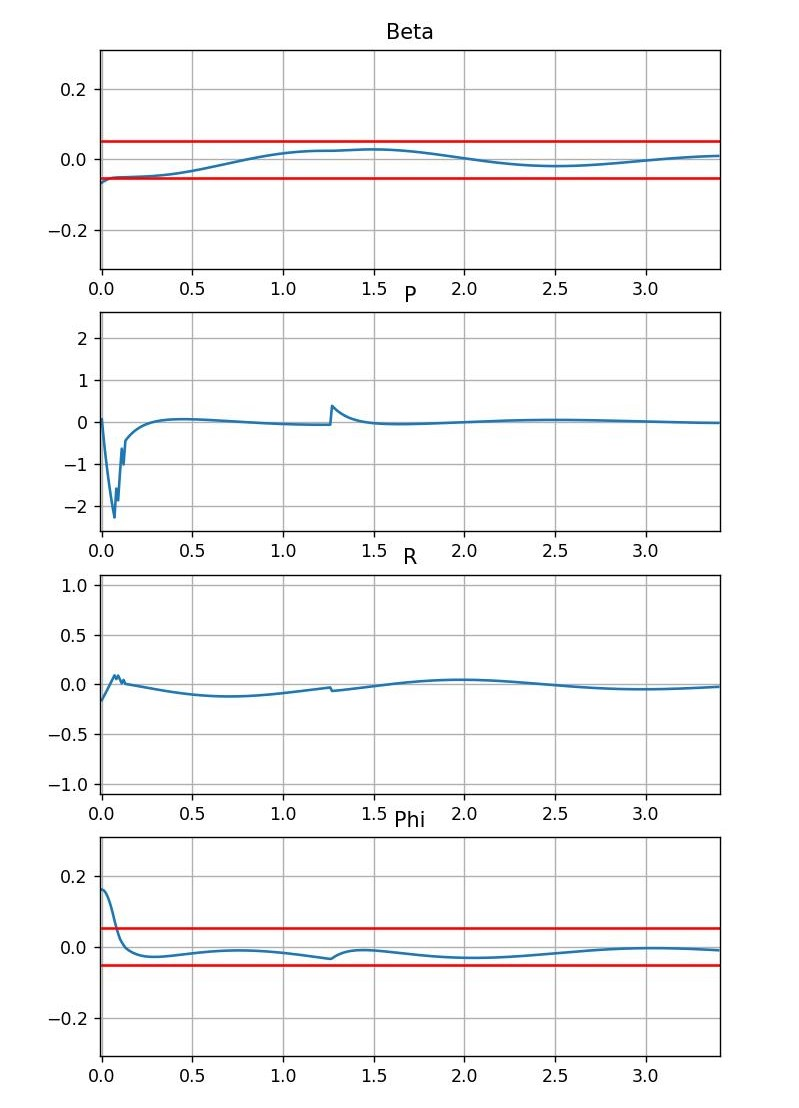
\includegraphics[scale=.3]{Figs/tamp.jpg}
            \end{figure}
        \end{columns}
    \end{frame}

    \section{TRPO algorithm}
    \begin{frame}
        \frametitle{\secname}

        \begin{itemize}
            \item TRPO optimal problem
            %%% ==================== TRPO optimal problem ====================
% The equation of TRPO optimal problem.
% Author: Wu, Po Hsun
% Date: September 03, 2022
%
\begin{equation} \label{eqn:TRPO_optimal}
\begin{aligned}
    \max_\theta\ & \hat{\mathbb{E}}_t\begin{bmatrix}\frac{\pi_{\theta}(a_t|s_t)}{\pi_{\theta_{\text{old}}}(a_t|s_t)}\hat{A}_t\end{bmatrix} \\
    \text{subject to}\ & \hat{\mathbb{E}}_t\begin{bmatrix}\text{KL}\begin{bmatrix}\pi_{\theta_{old}}(\cdot|s_t),\, \pi_{\theta}(\cdot|s_t)\end{bmatrix}\end{bmatrix} \leq \delta
\end{aligned}
\end{equation}

            \item \href{https://optimization.mccormick.northwestern.edu/index.php/Trust-region_methods}{Trust Region method} is to solving nonlinear problem
            %%% ==================== Trust region method ====================
% The equation of Trust region method.
% Author: Wu, Po Hsun
% Date: September 04, 2022
%
\begin{equation}
\begin{aligned}
    \min\ &m_k(p) = f_k+g_k^Tp+\frac{1}{2}p^TB_kp\\
    \text{subject to}\ &\|p\| \leq \Delta_k
\end{aligned}
\end{equation}


        \end{itemize}
    \end{frame}

    \section{PPO algorithm}
    \begin{frame}
        \frametitle{\secname}

        \begin{itemize}
            \item PPO(Proximal Policy Optimization) is upgrade from TRPO(Trust Region Policy Optimization)
            \item PPO optimal problem
            %%% ==================== PPO clip method ====================
% The equation of PPO using clip method.
% Author: Wu, Po Hsun
% Date: September 03, 2022
%
\begin{equation} \label{eqn:PPO_clip}
    \min_\theta\ \hat{\mathbb{E}}_t \left[\min\left(\frac{\pi_{\theta}(a_t|s_t)}{\pi_{\theta_\text{old}}(a_t|s_t)}\hat{A}_t,\,\text{clip}\left(\frac{\pi_{\theta}(a_t|s_t)}{\pi_{\theta_\text{old}}(a_t|s_t)},\, 1-\epsilon,\, 1+\epsilon\right)\hat{A}_t\right)\right]
\end{equation}


            clip function is to set the policy change inside $\left[1-\epsilon, 1+\epsilon\right]$
        \end{itemize}
    \end{frame}

    \section{Architecture}
    \begin{frame}
        \frametitle{\secname}

        \begin{figure}
            \centering
            %%% ==================== RLC_architecture ====================
% The figure of Reinforcement Learning policy architecture.
% Author: Wu, Po Hsun
% Date: May 28, 2022
%
\tikzstyle{circlenode}=[circle, draw=black, thick, minimum size=1mm]
\tikzstyle{squarednode}=[rectangle, draw=black, thick, minimum size=0mm, font=\footnotesize]

\begin{tikzpicture}[
    ->, >={latex},
    node distance=0.5cm,
    every state/.style={thick}
    ]
    % ---------- Nodes ----------
    \node[]             (input)                                 {$r(t)$};
    \node[circlenode]   (sum)           [right=of input]        {};
    \node[squarednode]  (policy)        [right=of sum]          {Neural Network};
    \node[squarednode]  (sampler)       [right=of policy]       {sampler};
    \node[squarednode]  (plane)         [right=of sampler]      {Plane};
    \node[]             (output)        [right=of plane]        {$y(t)$};
    \node[squarednode]  (RL_algorithm)  [above=of policy]       {RL Algorithm};

    % ---------- Lines ----------
    \draw[] (input.east) -- (sum.west);
    \draw[] (sum.east) -- (policy.west);
    \draw[] (policy.east) -- (sampler.west);
    \draw[] (sampler.east) -- (plane.west);
    \draw[] ($(plane.east)+(0.2,0)$) -- ++(0,-1) -| ($(sum.south)$);
    \draw[] (plane.east) -- (output.west);

    \draw[] (RL_algorithm.south) -- (policy.north);
    \draw[] (plane.north) |- (RL_algorithm.east);
    \draw[] ($(sum.east)+(0.2,0)$) |- (RL_algorithm.west);

    % ---------- Symbols ----------
    \node[right] at ($(sum.south)+(0,-0.2)$)            {$-$};
    \node[above] at ($(sum.west)+(-0.2,0)$)             {$+$};
    \node[above] at ($(RL_algorithm.east)+(0.4,0)$)     {$R(t)$};
    \node[above] at ($(RL_algorithm.west)+(-0.4,0)$)    {$e(t)$};
    \node[above] at ($(policy.east)+(0.4,0.2)$)           {$p(t)$};
    \node[above] at ($(sampler.east)+(0.4,0.2)$)          {$u(t)$};

    % ---------- Legend ----------
    \node[right, align=left] at (output.east) {
        $r(t)$: reference \\
        $y(t)$: state \\
        $e(t)$: error \\
        $R(t)$: reward \\
        $p(t)$: probability \\ \hspace{2em} of actions \\
        $u(t)$: control
    };

\end{tikzpicture}

        \end{figure}
    \end{frame}

\end{document}